% !TEX root = ../../main.tex


\begin{figure}[tb]
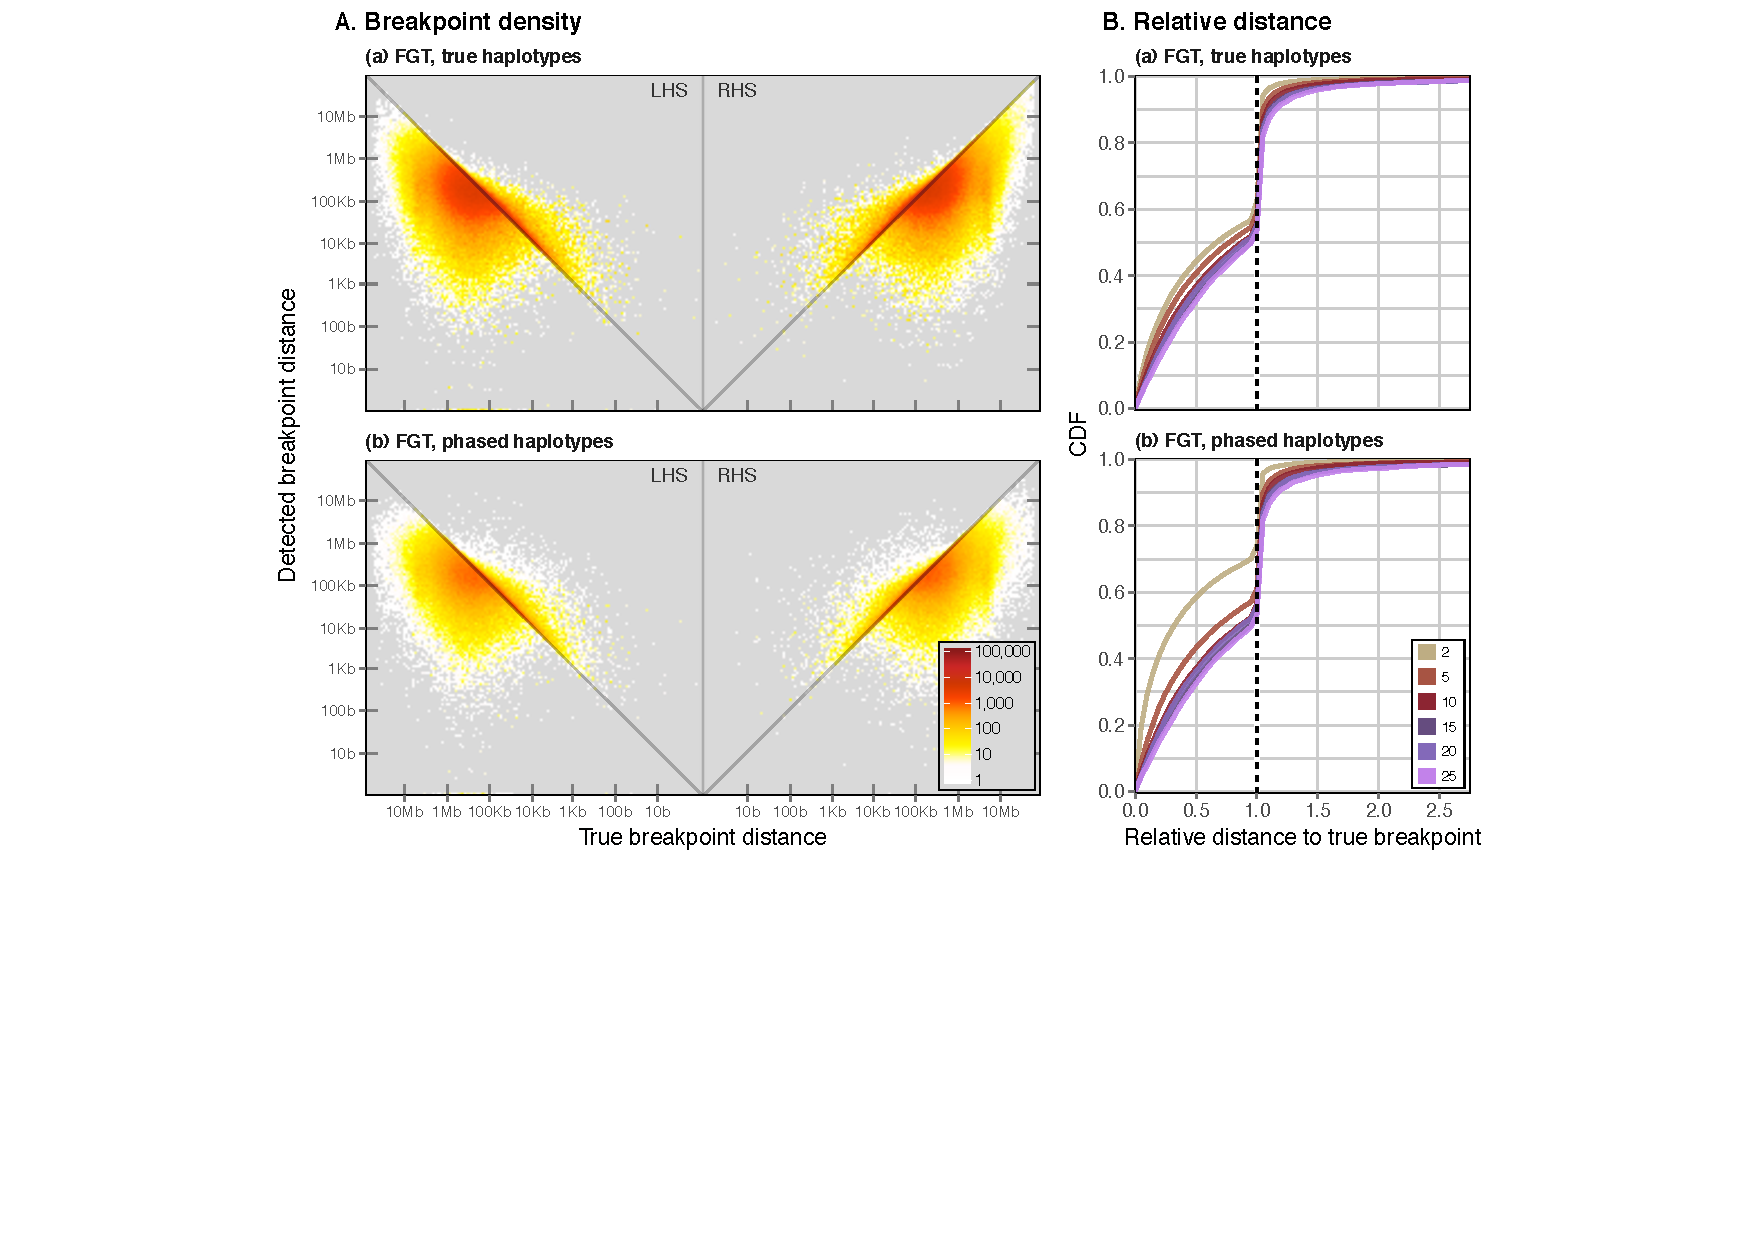
\includegraphics[width=\textwidth]{./img/ch3/beagle_break_tru}
\Caption{Accuracy of breakpoint detection in simulated data using Refined IBD in Beagle~4.1}
{Results are shown for \n{1} million randomly selected shared haplotype segments, after removing boundary cases in either the detected or true segments.
Segments were inferred using the \gls{fgt} on true haplotypes \textbf{(a)} and phased haplotypes \textbf{(b)}, as well as the \gls{dgt} on genotype data \textbf{(c)}.
Panel~\textbf{(A)} shows the density of detected breakpoints in relative distance to the focal and true breakpoint sites.
For each detected breakpoint, its physical distance to the focal site was divided by the distance between the corresponding true breakpoint and the focal site, such that values $<1$ indicate underestimation and $>1$ overestimation of the true distance (dashed line).
Panel~\textbf{(B)} provides a heatmap representation of a scatter plot, comparing physical distances between focal site and true breakpoint (x-axis) and detected breakpoint (y-axis).
Along each axis, distances were pooled into \n{200} bins (on log scale)
and the resulting $200^2$ squares were colour-coded for the number of  intersecting true and detected breakpoints, where grey indicates zero.
Segment breakpoints to the left (\emph{LHS}) and right-and side (\emph{RHS}) of the focal position are shown separately.}
{fig:beagle_break_tru}
% \vspace{-5pt}
% \hrulefill%
\end{figure}
